%!TEX program = xelatex
\documentclass[letterpaper,12pt]{exam}
\usepackage{../videoNotes}
\usepackage{xcolor}
\usepackage[dvipsnames]{xcolor}
\usepackage{soul}
\usepackage{tabulary}
\usepackage{fontspec}

\usepackage{draftwatermark}
\SetWatermarkText{Draft}
\SetWatermarkScale{1.5}
\SetWatermarkColor{red!20}

\newcommand{\unit}{Unit 09}
\pagestyle{headandfoot}
\firstpageheader{CSC 264 \semester\ \  \unit}{}{Name: $\rule{6cm}{0.15mm}$}
\runningheader{CSC 264 \semester}{\unit}{Page \thepage\ of \numpages}
\firstpagefooter{}{}{}
\runningfooter{}{}{}

\begin{document}

%\underconstruction

\par{\fontfamily{qzc}\selectfont\textbf{}}
\begin{questions}

\section*{\unit\_010 -- LEA }
\begin{samepage}
    \question What does LEA stand for?
    \vspace{5mm}
\end{samepage}
\par
\begin{samepage}
    \question How does the SYNTAX of the LEA instruction compare to the SYNTAX of the MOV instruction?
    \vspace{5mm}
\end{samepage}
\begin{samepage}
    \question How does the MEANING of the LEA instruction compare to the MEANING of the MOV instruction?
    \vspace{5mm}
\end{samepage}
\par
\begin{samepage}
    \question The following image is from the ddd debugger.  It shows the memory contents after lines 13 and 14 of the code were executed.  Why are the contents of r11 and r12 different?
   \begin{center}
    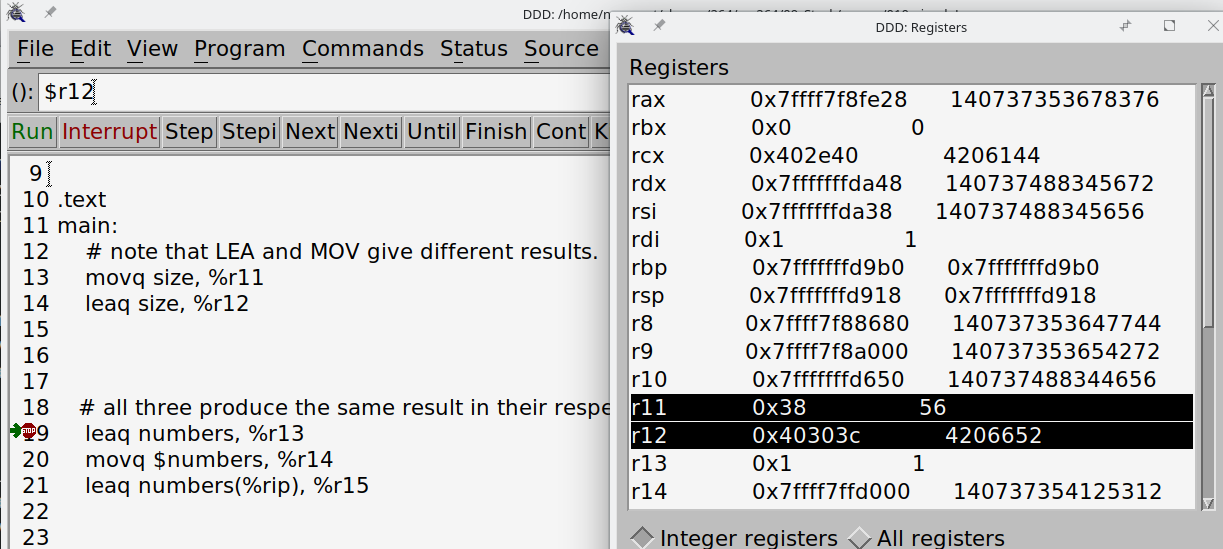
\includegraphics{../../09_Stack/images/010_LeaVsMov.png}
   % \includegraphics{../images/unit09_010_LeaVsMov.png}
   \end{center}
   \vspace{5mm}
\end{samepage}
\par
  
%----------------------------------
\end{questions} 
%footer
\begin{center}
    \rule{0.667\textwidth}{.8pt} %End of section
\end{center}


If you have any lingering questions or problems, please write them here or see me.
\vfill
\begin{center}
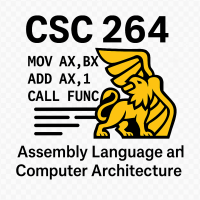
\includegraphics{../csc264Logo}
\end{center}
\end{document} 